\begin{figure}
  \centering
  \begin{subfigure}[htpb]{0.8\textwidth}
   \centering
   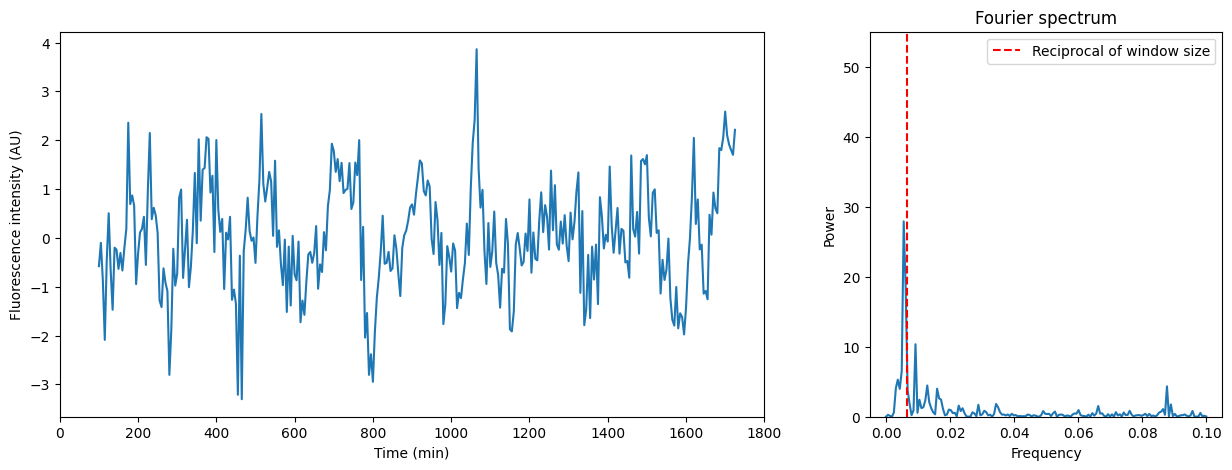
\includegraphics[width=\textwidth]{fft_slidingwindow}
   \caption{
   }
   \label{fig:analysis-slidingwindow-movavg}
  \end{subfigure}

  \begin{subfigure}[htpb]{0.8\textwidth}
   \centering
   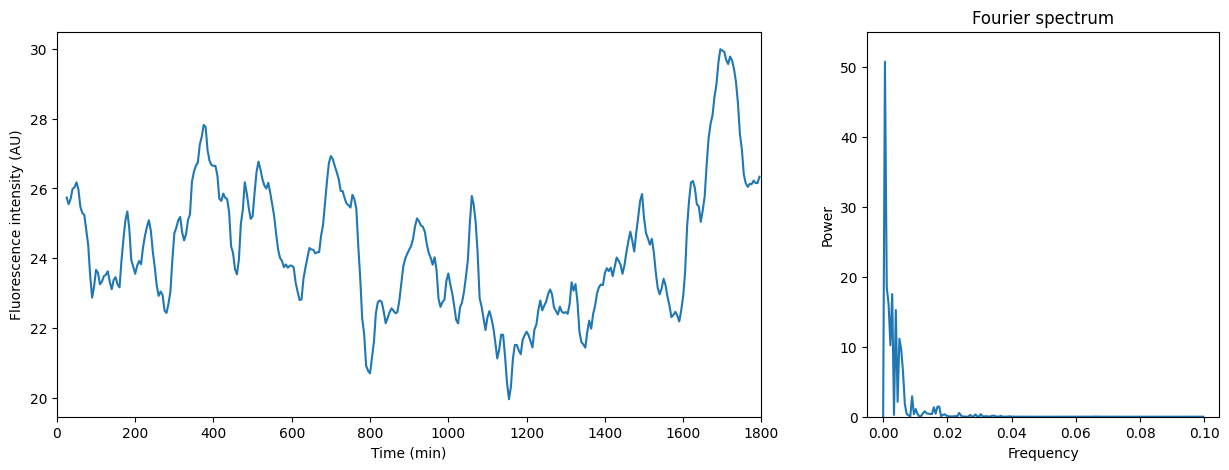
\includegraphics[width=\textwidth]{fft_savgol}
   \caption{
   }
   \label{fig:analysis-slidingwindow-savgol}
  \end{subfigure}

  \caption{
    (Left panels) Raw time series with trends, (middle panels) processed time series, and (right panels) Fourier spectra to demonstrate
    \textbf{(\ref{fig:analysis-slidingwindow-movavg})}
    using a moving average (window size 30), and
    \textbf{(\ref{fig:analysis-slidingwindow-savgol})}
    using a Savitzky-Golay filter (window size 7, polynomial order 3)
    to remove trends.
  }
  \label{fig:analysis-slidingwindow}
\end{figure}

Another caveat of this classifier lies in its sole tuning parameter, the false discovery rate, which affects the proportion of time series classed as oscillating.
To optimise the false discovery rate, labels of whether a time series is oscillatory were needed; if the labels are human-defined, as was the case in this section, any optimised false discovery rate would have low reliability.
Alternatively, a more reliable ground truth could be provided by an experiment expected to result in time series that are not oscillatory.

%[CONFIRM IMPORTANCE VIA RECURSIVE FEATURE ELIMINATION, USING RANDOM FOREST?]
Furthermore, Fig.\ \ref{fig:analysis-svc-catch22} suggests that the \texttt{FC\_LocalSimple\_mean3\_stderr} feature (represented as feature 9) is important for the classifier.
% Equation?
This feature is defined as the error based on using the mean of the previous three time points to predict each time point in the time series; time series that are more predictable should have low values of this feature.
Therefore, it is reasonable that oscillatory time series have higher values of this feature --- at any given time in the time series, the value changes substantially after three time points.
This is in contrast to noisy, non-oscillatory time series.

To assess the performance of a graph-based clustering method in identify clusters in time series data, I represented a dataset of time series as a graph before using modularity clustering to identify clusters.
Fig.\ \ref{fig:analysis-clustering-modclust} illustrates this process, specifically:
\begin{enumerate}
  \item \emph{Constructing a graph representation:}
        Each time series was represented as a vector of features in $n$-dimensional space, where $n$ is the length of the vector.
        Here, I represented each time series with a vector of 22 features using \textit{catch22}.
        The cosine distances between each pair of vector was computed, and became the edge weights of a complete graph with each time series as a node.
  \item \emph{Pruning:}
        The complete graph was pruned by deleting edges, so that each node had at least $k$ neighbours.
        Here, $k=10$.
  \item \emph{Modularity clustering:}
        Modularity clustering was performed on the graph to partition the pruned graph into communities.
        In this step, I used the Leiden algorithm \parencite{traagLouvainLeidenGuaranteeing2019}.
\end{enumerate}
